\Chapter{Introduction}
\label{Introduction}
\section{Fondamentaux de la physique des plasmas}

\emph{Le plasma}. Le plasma est souvent considéré un peu équivoquement comme le
quatrième état de la matière. Dans notre environnement proche, nous avons pris
conscience de son existence à travers les phénomènes de flammes, d'éclairs,
d'aurore boréales ou d'arc électriques. Mais à des conditions de pressions et de
températures différentes de celles de notre atmosphère terrestre, il est
omniprésent : plus de 99\% de la matière connue est sous cette forme.

Une définition plus adaptée du plasma est celle d'un gaz conducteur. Une partie
des atomes le composant est ionisée, donnant naissance à une population
d'électrons libres et d'ions de différentes espèces. Ces populations permettent
alors le transport de courant et, sensibles aux forces électromagnétiques,
influencent fortement le comportement global du plasma en provoquant des
phénomènes collectifs, non-linéaires et turbulents.

Le plasma et son comportement sont décrits par la théorie de la physique des
plasmas. Elle intègre les connaissances de nombreux domaines, tels que la
physique statitique, l'électromagnétisme, ou encore la dynamique des fluides.

\subsection{Les paramètres plasmas}
Les plasmas se présentent donc comme des gaz dont le comportement est influencé
de manière non négligeable par une population d'électrons libres $n_e$.
Les plasmas se caractérisent de plus par l'agitation moyenne de ses particules,
mesurée par la température électronique $T_e$.
La figure \ref{zoologie}, issue du livre du National Research
Council\cite{national1995Plasma}, représente une classification des plasmas en
fonction de ces deux paramètres principaux qui vont influer sur la dynamique du
transport de courant.
La théorie présentée dans la suite de cette thèse ne concerne que les plasmas
dits classiques :
\begin{itemize}
  \item les plasmas naturels peu dense tels que l'espace interstellaire,
  le vent solaire, la magnétosphère, et l'ionosphère
  \item les plasmas naturels denses tels que les éclairs et les étoiles
  \item les plasmas industriels, de laboratoire, et thermonucléaires
\end{itemize}
\begin{figure}[htbp]
\centering
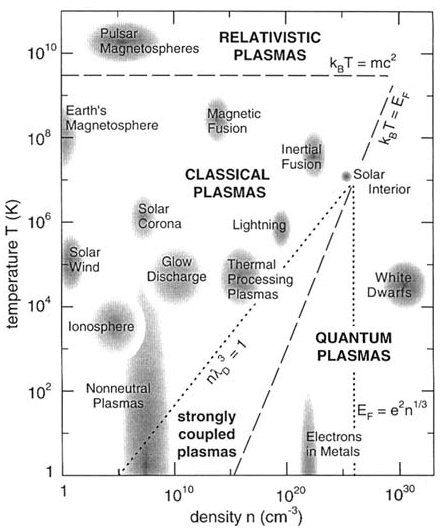
\includegraphics[height=80mm,width=64mm]{figures/zoologie.png}{\caption{Classification
de différents plasmas en fonction de $n_e$ et $T_e$.}\label{zoologie}}
\end{figure}

Dans ces plasmas, le dégré d'ionisation $\alpha$ est donné par le rapport
entre la densité électronique $n_e$ et la densité de gaz $n_g$ :
\begin{equation}
\alpha=\frac{n_e}{n_e+n_g}
\end{equation}
Cette fraction va définir l'importance de l'interaction entre les particules
neutres et les particules chargées. Cependant, même à très faible $\alpha$,
l'apparition d'une population de porteurs de charge va modifier les caractéristiques et la
dynamique du plasma.

L'ionisation du gaz suit l'évolution de la température électronique $T_e$ qui
mesure l'agitation thermique des électrons. Densité et température
électronique permettent de définir le paramètre plasma:
\begin{equation}
\label{1-paramPlasma}
\Gamma=\frac{<E_p>}{<E_c>}=\frac{e^{^2}n_e^{^{1/3}}}{\varepsilon_{_0}
eT_e}
\end{equation}
Le paramètre plasma représente le ratio entre l'énergie thermique des
électrons et leur énergie potentielle électrostatique coulombienne \emph{ie.}
l'agitation thermique desordonnée contre les forces d'interactions
coulombiennes structurantes.

Les plasmas classiques (ou cinétiques) sont caractérisés par
$\Gamma\ll 1$. Ils ont une population d'électrons assez espacée et/ou une
température suffisamment élevée.

\subsection{Echelles et phénomènes collectifs}
La dynamique d'un plasma résulte du couplage entre le mouvement des
particules chargées et les forces électromagnétiques $\mathbf
F=q_s(\mathbf E+ \mathbf v_s\times\mathbf B)$
présentent ou qui se forment dans le système.
Elle se décompose principalement sur deux échelles de temps : la première
phase correspond à l'équilibre électrostatique, où une
quasineutralité s'établit. Dans une deuxième phase, l'évolution quasineutre du
plasma, plus lente, tend à former un équilibre entre les particules et la valeur locale
et instantanée des champs de force extérieurs.
.
\subsection{Quasineutralité}
Le processus le plus rapide est lié à
l'équilibre microscopique électrostatique qui s'opère
entre l'agitation thermique et l'interaction coulombienne des particules. Les
ions et les électrons issus de l'ionisation se réorganisent pour écranter
leur champ électrique individuel et former ainsi un ensemble électriquement neutre.
Cette dynamique est essentiellement portée par les électrons et décrite aux plus petites
échelles spatiotemporelles par le principe fondamental de la dynamique et la loi de Boltzman-Poisson :
\begin{align}
\label{1-PFD}
m_e\frac{\partial \mathbf{v}_e}{\partial t}=-e\mathbf E
\;\;\;\;\;\;\text{et}\;\;\;\;\;\;
\nabla\cdot\mathbf{E}=\rho\varepsilon_{_0}^{\moinsun}
\end{align}
où $m_e$ est la masse de l'électron, $\mathbf{v}_e$ sa vitesse,
$e$ la charge élémentaire, $\rho=e\,(n_i-n_e)$ la densité de charge,
résultant de la différence entre la densité ionique et la densité
électronique.
Les échelles fondamentales définies par \ref{1-PFD} sont alors la pulsation
plasma et la longueur de Debye\footnote{Le nombre de particules présentes
dans la sphère de rayon $\lambda_D$ définit un paramètre adimensionné
semblable au paramètre plasma (Eq.\ref{1-paramPlasma}). Un
grand nombre de particules dans la sphère de Debye $n\lambda_D^3\gg1$
définit un plasma idéal, où le phénomène d'écrantage électrique est
dominant.}, reliée par l'intermédiaire la vitesse thermique :
\begin{equation}
\omega_p\left[\left(\frac{n_{_0}e^{^2}}{\varepsilon_{_0}
m_e}\right)^\text{\textonehalf}
\right]\cdot\lambda_D\left[\left(\frac{\varepsilon_{_0}
eT_e}{n_{_0}e^{^2}}\right)^\text{\textonehalf}\right]
=v_{th}\left[\left(\frac{eT_e^{^{\phantom{1}}}}{m_e}\right)^\text{\textonehalf}\right]
\end{equation}

Au delà de ces échelles, le plasma est dans un état de \emph{quasi-neutralité}, ie. $n_e=n_i$.

Le système évolue ensuite sur cet équilibre par le biais de
\emph{phénomènes de transport} résultants de l'influence
globale des champs électromagnétiques et de la tendance à
l'homogénéisation du plasma par collisions entres particules.
Ces processus interviennent sur des échelles relativements
lentes et relativement grandes devant $\omega_p$ et $\lambda_D$ :
\begin{equation}
\tau\gg \omega_p^{\moinsun} \;\;\;\;\text{et}\;\;\;\;\tau v\gg\lambda_D
\end{equation}
$\tau$ étant le temps et $v$ la vitesse caractériques du processus de transport
considéré.
On parle alors de diffusion/convection de particules, de viscosité (transfert de
quantité de mouvement), de conductivité (transport de charges) ou encore de
conductivité thermique (transport de chaleur).

\subsection{Collisions}
Dans un plasma, les électrons, les ions et les atomes neutres sont constament en
mouvement les uns par rapports aux autres.
Au cours de leur déplacement, ces particules peuvent rentrer en collision avec d'autres
ou encore être déviées de leur trajectoire par l'action de la force
coulombienne. Ces interactions binaires directes entre particules, regroupées
sous le terme général de collisions, sont fondamentales dans la physique des plasmas.
Elles sont définies pour chaque couple d'espèces de particules et catégorisées suivant
leur nature élastique (dans le cas où la nature des particules en collision
reste inchangée) ou inélastique (dans le cas de l'ionisation, des
recombinaisons ou des processus d'exitation/desexitation , entraînant pour
chacun des cas des comportements spécifiques.




\textbf{Collisions élastiques}

\subsection{Plasma et champ magnétique}
%\begin{wrapfigure}{r}{0.50\textwidth}
%	\vspace{-5pt}
%
%	%
%	%
% \hspace{20pt}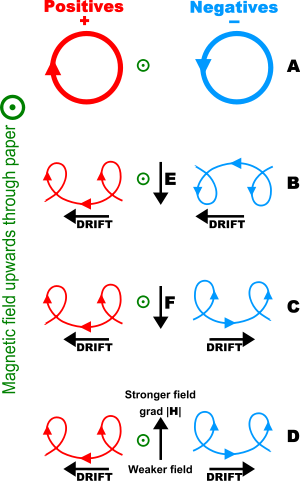
\includegraphics[width=0.40\textwidth]{figures/particleDrifts.png} \hspace{20pt}\caption{Mouvement cyclotronique et de dérive des particules
%	dans un champ magnétique.}\label{particleDrifts}
%	 \vspace{-20pt}
%\end{wrapfigure}
\begin{figure}
\centering
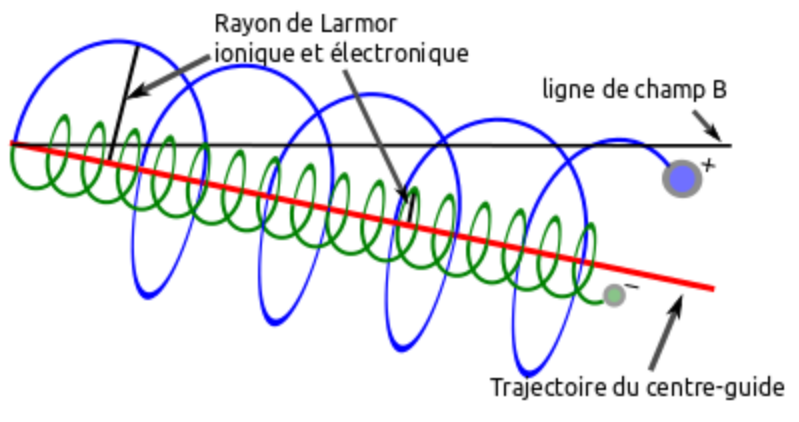
\includegraphics[width=0.8\textwidth]{figures/mouvementCyclotron.png}
{\caption{Mouvement cyclotronique des particules autour des lignes de champ
magnétique.}\label{1-particleDrifts}}
\end{figure}
La présence d'un champ magnétique influence aussi fortement le transport global qui
se met en place dans les plasmas. Sous l'action de la force de Lorentz, les particules
chargées sont en rotation autour des lignes de champ magnétique. En l'absence de force
extérieure, les particules sont confinéesLeur mouvement peut alors
se décrire par trois composantes (cf. figure \ref{1-particleDrifts}) :
\begin{itemize}
  \item Un déplacement parallèle aux lignes de champ, de l'ordre de la vitesse
  thermique de l'espèce, $v_\para\approx c_s=(eT_s/m_s)^{\text{\textonehalf}}$
  \item Le mouvement cyclotronique, rotation rapide de la particule
  autour des lignes de champ magnétiquedans le plan perpendiculaire aux lignes
  de champ
  \item Une vitesse de dérive,
\end{itemize}

Dans suite de cette thèse, nous allons étudier la dynamique électrique d'un
plasma en milieu magnétisé , ie. ou les structures et la dynamique
essentiellement reliée aux variations du champ électrique.
\section{Description fluide d'un plasma}

\subsection{De la statistique au fluide}
$$\partial_tf_s+\mathbf{v}_s\cdot\vec\nabla_\mathbf{r}f_s+
\frac{\mathbf{F}_s}{m_s}\cdot\vec\nabla_{\mathbf{v}_s}f_s
=\partial_tf_{|_{coll}}$$ 
Braginskii equations
$$M^{(k)}_s=\int_{-\infty}^{\infty}\mathbf{v}_s^kf_sd\mathbf{v}$$
\subsection{Conservation de la matière}
$$n_s=\int f_sd\mathbf{v}$$

\subsection{Conservation de l'impulsion}
$$n_s\mathbf{v}_s=\int \mathbf{v}_sf_sd\mathbf{v}$$
\subsection{Conservation de l'énergie}
\subsection{Conservation de la chaleur}
\section{Les gaines électrostatiques}
Les gaines électrostatiques sont des structures non-neutres qui se
développent à la frontière entre un plasma et un objet. Elles apparaissent
spontanément du fait de la plus grande vitesse des électrons par rapport à
celle des ions. D'une taille de l'ordre de quelques longueurs de Debye $\lambda_D$,
L'interaction dite plasma-paroi est une branche à part entière de la physique des plasmas.
En effet, au contact d'un milieu extérieur, que ce soit un obstacle matériel
ou un gaz ambiant, le plasma perd sa quasineutralité.
\subsection{Physique de la prégaine}
\subsection{Physique de la gaine}
\subsection{Gaine dans les plasmas magnétisés}
\subsection{Problématique de la gaine parallèle aux lignes de champ}

\section{Les décharges plasma basse-pression}
\subsection{Création de la décharge, rôle des électrons}
Dans les plasmas basse-température industriels et de laboratoires, qui possédent
un faible degré d'ionisation, ou dans l'ionospère, la dynamique du plasma est dominée par
la perte de quantité de mouvement dûe à l'ionisation la force de friction avec le gaz.
Electrical breakdown, Townsend avalanche,
\subsection{Trasport des ions et champ ambipolaire}
\begin{equation}
\label{derivediffusion}
\end{equation}
\subsection{Equations de dérive-diffusion magnétisées}

\section{Les plasmas de bord des tokamaks}
Lawson criteriom, strongly magnetized
\subsection{La fusion et les tokamaks}
\subsection{Le plasma de la Scrape-of-Layer}
\subsection{Les vitesses de dérives}
\label{vitessesDerive}
\section{Les modèles numériques}
L'étude de phénomènes complexes
%\begin{figure}[htbp]
%	\centering
%	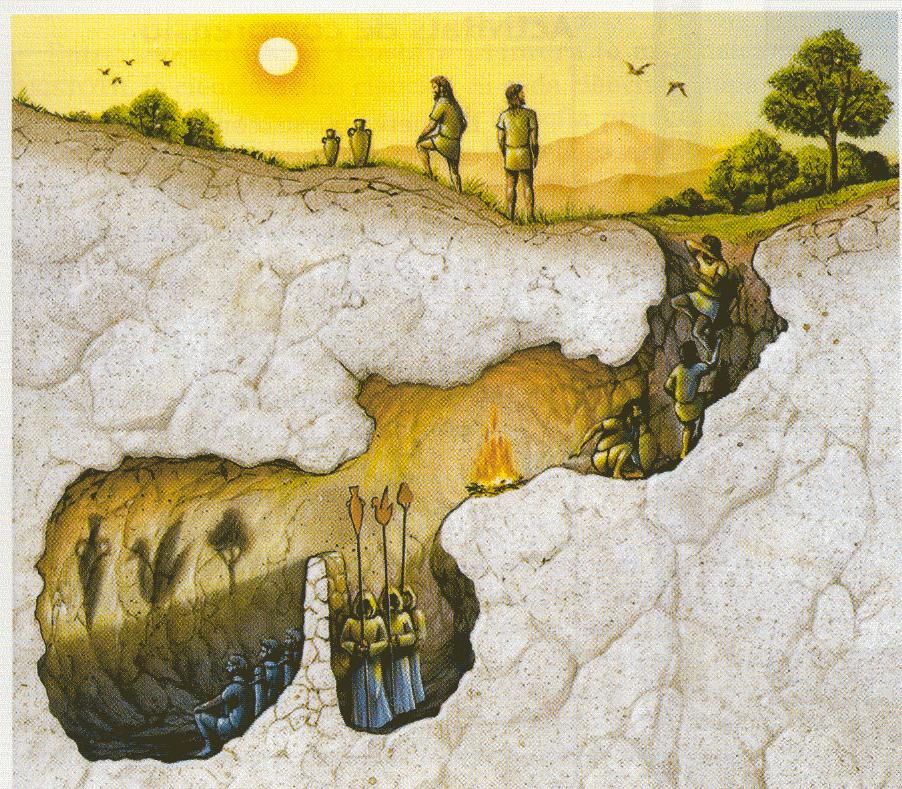
\includegraphics[height=64mm]{figures/cave.jpg}
%	{\caption{La caverne des idées.}\label{caverne}}
%\end{figure}
%\begin{figure}[htbp]
%
%			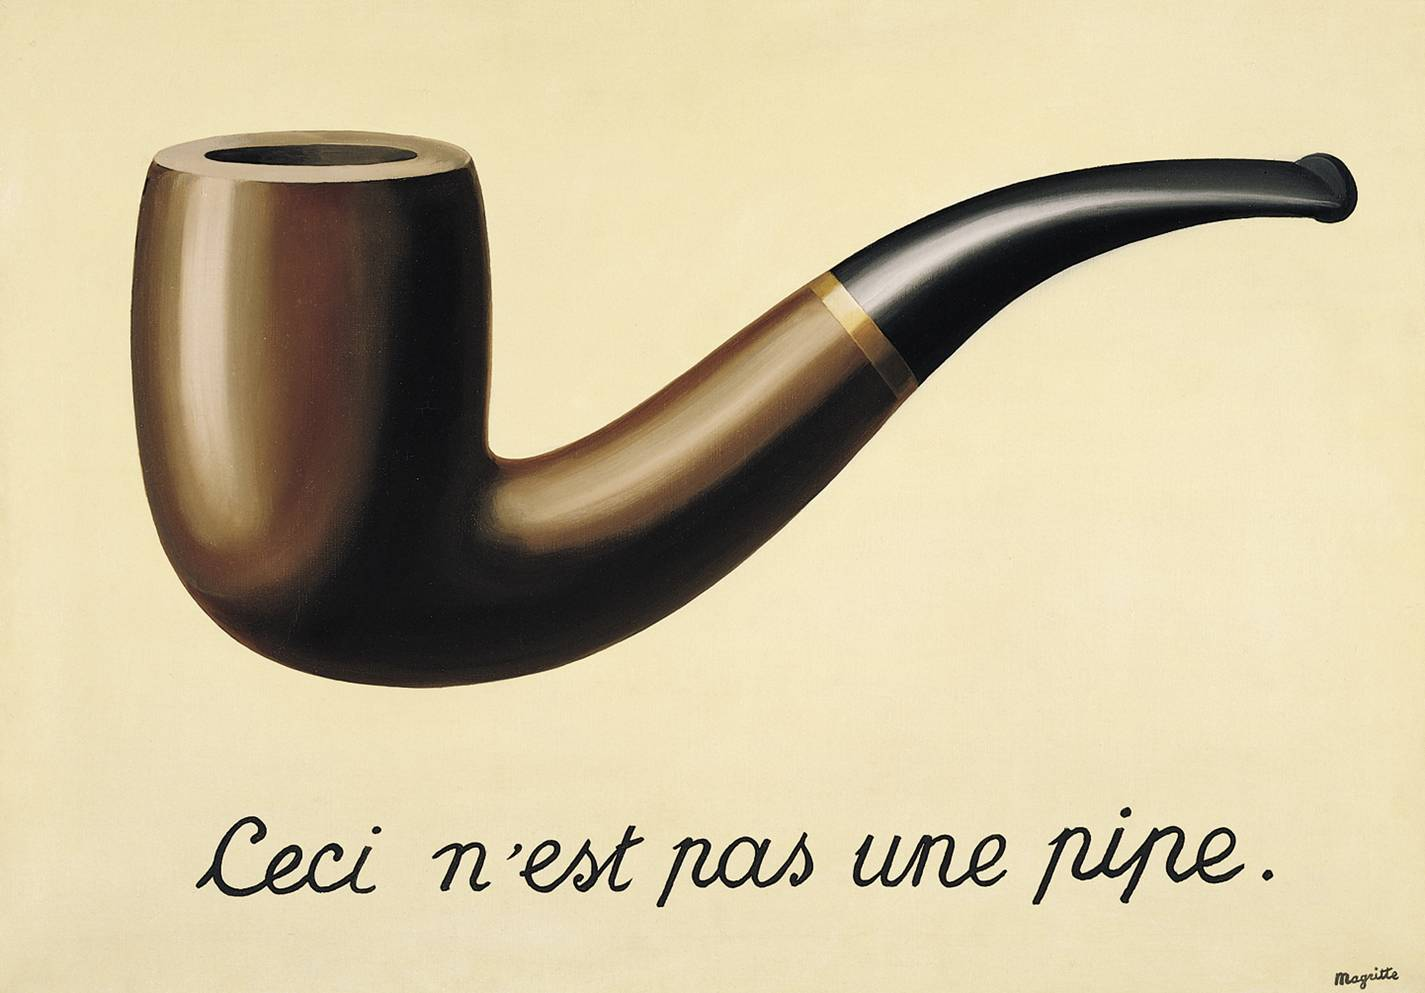
\includegraphics[height=40mm]{figures/Magritte.jpg}
%			{\caption{Magritte. La trahison des images.}\label{magritte}}
%		\end{figure}





